\usetikzlibrary{decorations.pathmorphing}

% Define spring style
\tikzset{
    spring/.style={
        decorate,
        decoration={
            coil,
            aspect=0.4,
            segment length=3mm,
            amplitude=3mm
        }
    },
    damper/.style={
        thick
    }
}

\begin{document}
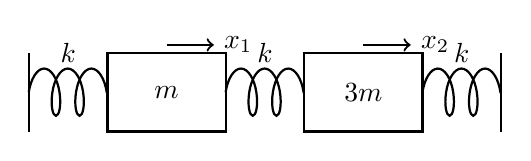
\begin{tikzpicture}[thick]

% Left wall
\draw (-2,0.5) -- (-2,-0.5);

% First spring
\draw[spring] (-2,0) -- (-1,0);

% First mass (m)
\draw[fill=white] (-1,-0.5) rectangle (0.5,0.5);
\node at (-0.25,0) {$m$};
\draw (-0.25,0.6) [->] -- ++(0.6,0) node[right] {$x_1$};

% Middle spring
\draw[spring] (0.5,0) -- (1.5,0);

% Second mass (3m)
\draw[fill=white] (1.5,-0.5) rectangle (3,0.5);
\node at (2.25,0) {$3m$};
\draw (2.25,0.6) [->] -- ++(0.6,0) node[right] {$x_2$};

% Right spring
\draw[spring] (3,0) -- (4,0);

% Right wall
\draw (4,0.5) -- (4,-0.5);

% Labels for springs
\node at (-1.5,0.5) {$k$};
\node at (1,0.5) {$k$};
\node at (3.5,0.5) {$k$};

\end{tikzpicture}
\end{document}
